\documentclass[12pt,a4paper,oneside]{article}
\usepackage{titlepic}
\usepackage[utf8]{inputenc}
\usepackage{graphicx}
\usepackage[left=1.1in,right=1.1in, top=1in, bottom= 1in]{geometry}
\usepackage{amsfonts}
\usepackage{amssymb}
\usepackage{amsmath}
\usepackage{fancyhdr}
\usepackage{hyperref}
\usepackage{etoolbox}
\usepackage[nottoc]{tocbibind}
\usepackage{appendix}
\usepackage{multicol}
\usepackage{leftidx}
\graphicspath{{figures/}}
\usepackage{ragged2e}
\usepackage{mathtools}
\usepackage{units}
\usepackage{float}
\usepackage{subcaption}
\usepackage{commath}
\usepackage{comment}

\usepackage{amsthm}
 
\theoremstyle{definition}
\newtheorem{definition}{Definition}[section]

\newtheorem{theorem}{Theorem}

\usepackage[none]{hyphenat} % Avoids to go out of margin

\usepackage{subfiles}

\usepackage{minted}
\usemintedstyle{manni}
\setminted{breaklines}

% --------------------------------------------- %

\title{Derp}	                                    % Title
\author{Author Name}				                % Authors separated by \\
\date{\today}									    % Date

% Font size of figure smaller than normal size:
\usepackage{caption}
\captionsetup[figure]{font=small}
%\captionsetup[table]{font=small}

%\usepackage{setspace} % double spacing
\linespread{1.2}

\makeatletter
\let\thetitle\@title
\let\theauthor\@author
\let\thedate\@date
\makeatother

\begin{document}

\begin{titlepage}
	\centering
	\vspace*{0.5 cm}
	\includegraphics[scale = 0.75]{figures/SapienzaLogo.pdf}\\[1.0 cm]	% University Logo

	{ \fontsize{20.74pt}{18.5pt}\selectfont\bfseries \thetitle \par } % Title

	\vspace*{0.25cm}
	\textsc{\Large Blockchain and Distributed Ledger Technologies 2022}\\[0.5 cm] % Course Name

	\vspace*{2.6cm}
	\hspace{3em}
	\begin{minipage}{0.3\textwidth} % 0.4
		\begin{flushleft} \large
			\textbf{Andrea Reale}\\
			2003188\\
		\end{flushleft}
	\end{minipage}~
	\hspace{3em}
	\begin{minipage}{0.3\textwidth} %0.4
		\begin{flushright} \large
			\begin{minipage}{1\textwidth}
				\begin{flushleft} \large
					\textbf{Matteo Gioia} \\
					1995989
				\end{flushleft}
			\end{minipage}
		\end{flushright}
	\end{minipage}\\[3.85 cm]

	\vspace{8cm}
	\rule{\linewidth}{0.2 mm} \\[0.3 cm]
	Academic Year 2022/2023
\end{titlepage}

\newpage
\tableofcontents
\newpage


%glossary in latex
%context: a context in phoenix is a module that is used to group related functionality.


\section{Introduction}

The rise of e-commerces revolutionized the way we buy and sell products. Before the creation of such platforms, there was no way to verify the quality of a product, as gathering feedback from previous customers was pretty much impossible.
This issue became one of the main selling points of e-commerces, as they provided a way for users to share their experience with a product and for others to make an informed decision before buying it.
However, the lack of a centralized authority to verify the authenticity of the reviews has led to the proliferation of fake reviews. For example, it is not uncommon for vendors to ask to leave fake reviews in exchange for money or a free product, or for users to leave negative feedbacks in order to boycott a specific vendor. On top of that, there is no way to verify whether the content of the review is what the original poster had actually written. \\
The goal of D.E.R.P. is to address all of these challenges while building a platform that incentivizes its customers to leave honest reviews and interact with the website.

\paragraph{Responsibilities} The development of the app (backend, frontend, smart contract) was carried on by all team members equally. However, there are a few key elements which were personally ideated/curated by a specific team member, as listed below:
\begin{itemize}
	\item Andrea Reale: oracle to check whether user has bought news product, docker setup
	\item Matteo Gioia: documentation stub, slides
\end{itemize}

\paragraph{Outline of the report TO CORRECT} This report is organized as follows:
\begin{itemize}
	\item The first section provides a brief overview of the background of the project, including a brief introduction to the blockchain technology and the e-commerce domain.
	\item The second section describes the context of the DApp, including the main problems that we are trying to solve and the rationale behind the use of a blockchain.
	\item The third section describes the architecture of the DApp, including the functional requirements, the use-case diagrams, the sequence diagrams, the backend, the frontend and the smart contract.
	\item The fourth section describes the implementation details of the DApp, including visual examples.
	\item The fifth section describes the known issues of the DApp.
	\item The last section provides a conclusion of the project.
\end{itemize}

\section{Background}
% Blockchain: history, rationale, concepts...

\subsection{E-commerce}
% Application domain

\section{Context of the D-App}
% Aim of the DApp
The goal of D.E.R.P. is to solve the problem of fake reviews on e-commerce platforms. The main idea is to use a blockchain to store the reviews and verify their authenticity. Other features will include the possibility to interact with the reviews and customize the user profile. A full list of the features is available in the requirements section. \\
The main problems that we tackle are:
\begin{itemize}  
	\item Authenticity: the hash of the review should be stored on-chain, so that it's authenticity can be verified.
	\item Boycotting: users shouldn't be able to boycott a product by leaving fake reviews.
	\item Over the counter scams: vendors shouldn't be able to bribe users to leave fake reviews.
	\item Self promoting: vendors shouldn't be able to buy/generate reviews through fake accounts.
\end{itemize}

We also want to provide a place for users to customize their profile, such as a personal page. This will increase the engagement of the users and will incentivize them to keep interacting with the platform. \\
Ideally, this platform should solve entirely the problem of fake reviews, however we are aware that this is not possible unless other requirements are met. For an extensive list of know issues, please refer to the appropriate section. 

\subsection{Why using a blockchain?}

\subsection{Functional Requirements}

In this section we define a list of functional requirements for D.E.R.P.

\subsection{Tech stack}

The technology stack used in the project is the following:
\begin{itemize}
	\item \textbf{Backend}: Phoenix (Elixir framework), PostgreSQL (Database)
	\item \textbf{Frontend}: Phoenix, Javascript, Bootstrap5, Web3.js (interaction with smart contract), Alpine.js (dynamic frontend)
	\item \textbf{Smart contract}: Solidity, Truffle Suite, IPFS
	\item \textbf{Tooling}: Docker, Git
	\item \textbf{Fake shop}: Deno
\end{itemize}

The backend is written in Elixir and the CRUD were autogenerated with the help of the Phoenix framework. The frontend is also written in Phoenix and Javascript, and the interactions with the smart contract are handled with Web3.js. The smart contract is written in Solidity and it is deployed on a local node of the Ethereum blockchain, simulated with Truffle. \\
For what regards the tooling, we created 4 containers: one for the shop server, one for truffle, one for IPFS and one for PostgreSQL. Github was used for managing the code and the project.
For an extensive list of the libraries used in the project and for a quick startup guide, please refer to the github repository that can be found at this link \url{among.us}.

\newpage
\section{Architecture}

This section is dedicated to discussing the architectural details of the DApp. In particular, we will discuss the use-case diagrams, the sequence diagrams, the backend, the frontend and the smart contract. 

\subsection{Use-case diagrams}

% \begin{figure}[h]
%     \includegraphics[width=0.75\linewidth]{assets/Use Case Diagram.svg}
% \end{figure}

In this section we show the main use case diagram of our app. Since the interactions are relatively simple, we managed to fit everything in a single diagram. In fact, we only have 3 actors: the users (reviewers), the smart contract and the token themselves.

\begin{figure}[ht]
	\centering
	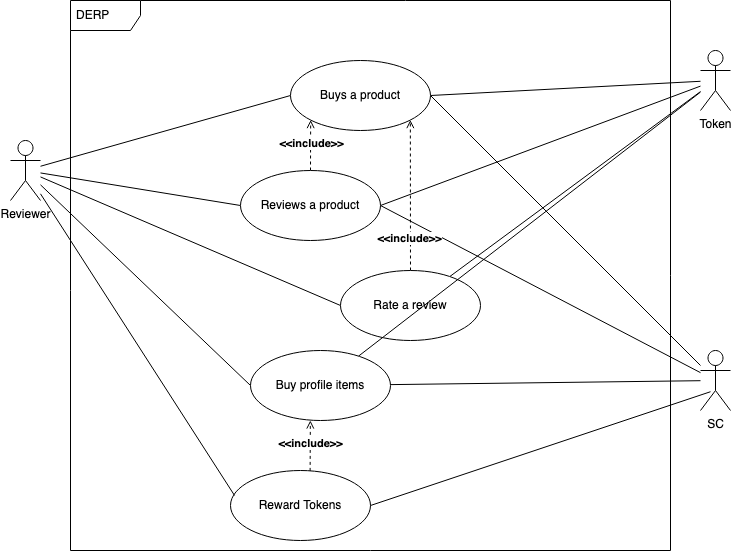
\includegraphics[scale=0.5]{figures/uc_drawio.png}
	\caption{Use case diagram}
	\label{fig:use_case}
\end{figure}

\subsection{Sequence diagrams}


\subsection{Backend}

The backend of D.E.R.P. is fully written in Elixir, using the Phoenix framework. It is responsible for scaffolding (handling authentication) and for saving part of the user information, since most of the data we use is on-chain (as we need proof of its authenticity). 

Before creating the backend, we had to decide how to structure the project. We came up with following ER diagram and used it to decide the main entities and the context of each one.

\begin{figure}[ht]
    \centering
    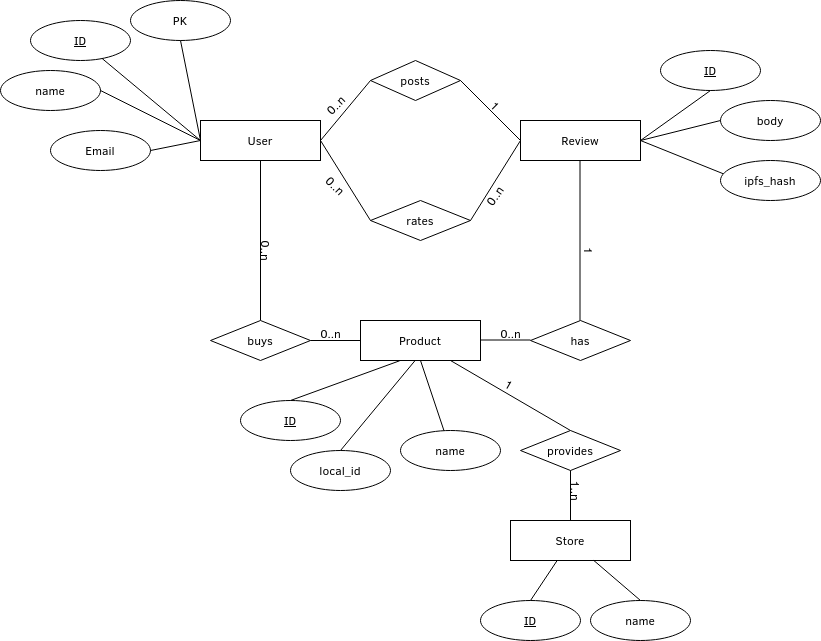
\includegraphics[scale=0.5]{figures/derp_er.drawio.png}
    \caption{Caption}
    \label{fig:my_label}
\end{figure}

To keep things organized, we created 4 contexts: 
\begin{itemize}
	\item \textbf{Accounts}: procedures related to user authentication.
	\item \textbf{Catalogue}: procedures related to stores/products.
	\item \textbf{Reviews}: procedures related to reviews.
	\item \textbf{Oracle}: procedures related to the oracle.
\end{itemize}

The contexts for Accounts, Catalogue and Reviews handle the usual CRUD operations (which weren't really needed as we fetch data from chain).
The context for the Oracle is the most complex, as it has to spawn 2 subprocesses that listen for events from the contract and it allows us to grant review tokens to the users that request them after buying a product from the shop. The 2 subprocesses are handled by elixir and will restart on their own if they crash. 

Here we include the (significant parts of the) oracle code.

\inputminted{Elixir}{event_handler.ex}
\inputminted{Elixir}{oracle.ex}

\paragraph{Why use a backend at all?} A case could be made that the backend is not really needed, as we could just use the smart contract to store all the data. However we do not need to verify the authenticity of all of the information used in the website (we mentioned user settings or preferences), and storing it on the chain would increase the price of the contract without any real benefit. Additionally, having a solid (pun intended) backend is a good choice for future development, as it gives the possibility to easily expand the website in the future. \\ 

\subsection{Frontend}

 The fronted for D.E.R.P. uses the Phoenix framework to render each webpage. To provide a better interaction, we also used Alpine.js  to handle events or refreshes and to fill data that was fetched from the contract or IPFS. We interacted with the smart contract through web3.js whenever a user had to make a transaction. For what regards the UI, we created a really basic design using Bootstrap 5.  \\

\subsection{Smart contract}

The smart contract for D.E.R.P. is written in Solidity and it is deployed on Truffle Suite. The main responsibilities of the contract are meant to fullfil most of the functional requirements, namely:
\begin{itemize} 
	\item store the reviews on-chain, grant authenticity;
	\item store the products and some information about them;
	\item store information about profile items and their prices;
	\item handle users' interaction with products (e.g. verify that a user has bought a product or claimed their review tokens);
	\item handle the interactions regarding review tokens and profile tokens.
\end{itemize}

Here is a full copy of all of the contract's functions.

\inputminted{Solidity}{Derp.sol}

To complete the interaction with the smart contract we also used IPFS. In fact, storing the reviews on-chain would be too expensive, so we decided to store them on IPFS and just store the hash. This way, we can verify the authenticity of the review and we can also retrieve the review text easily. We did a similar thing for the profile items too, in order to store less information on chain. \\

\section{Images} %TO MOVE

\section{Known issues}

% We can't prevent over the counter scams
% Stores are forced to use our API (can prevent adoption)

\section{Conclusion}

\newpage
%\printbibliography


\end{document}

